\documentclass[xetex,mathserif,serif]{beamer}
\usepackage{polyglossia}
\setdefaultlanguage[babelshorthands=true]{russian}
\usepackage{minted}
\usepackage{tabu}

\useoutertheme{infolines}

\usepackage{fontspec}
\setmainfont{FreeSans}
\newfontfamily{\russianfonttt}{FreeSans}

\definecolor{links}{HTML}{2A1B81}
\hypersetup{colorlinks,linkcolor=,urlcolor=links}

\tabulinesep=0.7mm

\title{Структурные паттерны}
\subtitle{Детали реализации}
\author[Юрий Литвинов]{Юрий Литвинов \newline \textcolor{gray}{\small\texttt{yurii.litvinov@gmail.com}}}

\date{08.04.2020г}

\begin{document}
    
    \frame{\titlepage}

    \section{Мост}

    \begin{frame}
        \frametitle{Паттерн ``Мост'' (Bridge)}
        Отделяет абстракцию от реализации

        Пример:
        \begin{itemize}
            \item Есть система, интерпретирующая программы для роботов
            \item Есть класс \textit{Sensor}, от которого наследуются \textit{SonarSensor}, \textit{LightSensor}, ...
            \item Связь с роботом может выполняться по USB или Bluetooth, а может быть, программа и вовсе исполняется на симуляторе
            \item Интерпретатор хочет работать с сенсорами, не заморачиваясь реализацией механизма связи
            \item Рабоче-крестьянская реализация --- \textit{USBLightSensor}, \textit{BluetoothLightSensor}, \textit{USBSonarSensor}, \textit{BluetoothSonarSensor}, ...
            \item Число классов --- произведение количества сенсоров и типов связи
        \end{itemize}
    \end{frame}

    \begin{frame}
        \frametitle{``Мост'', пример}
        \begin{center}
            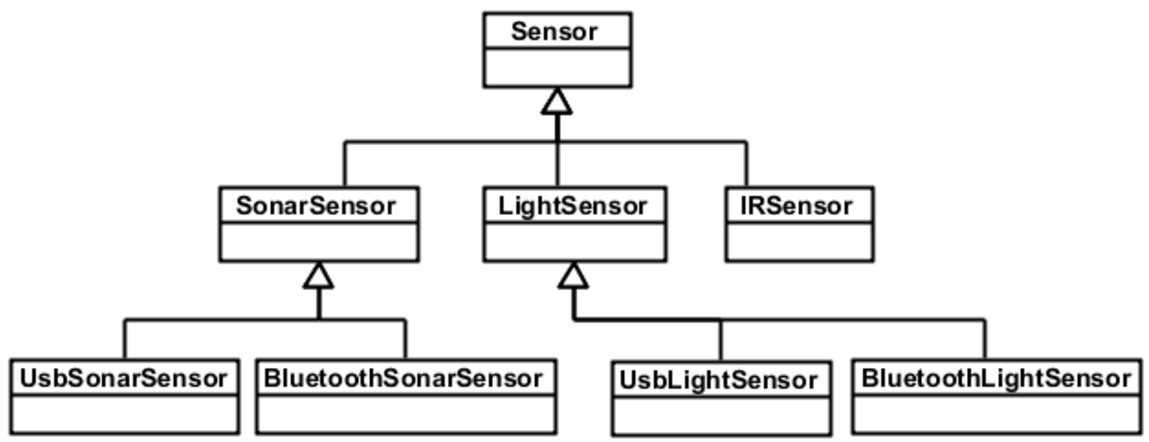
\includegraphics[width=0.7\textwidth]{noBridge.png}
            \Huge{$$\downarrow$$}
            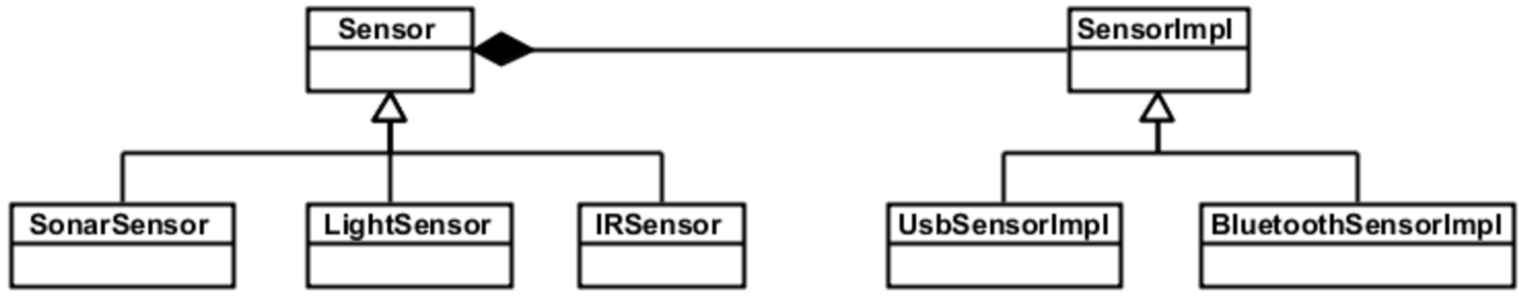
\includegraphics[width=0.7\textwidth]{bridge.png}
        \end{center}
    \end{frame}

    \begin{frame}
        \frametitle{``Мост'', общая схема}
        \begin{center}
            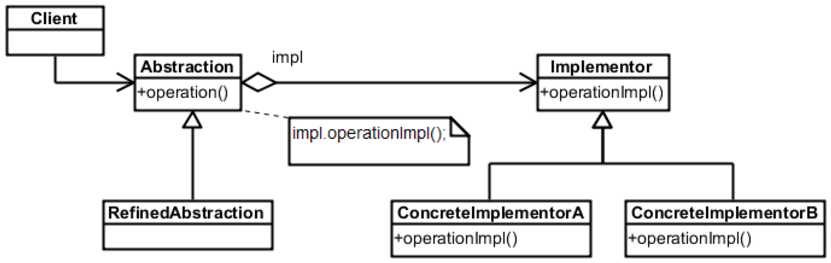
\includegraphics[width=0.7\textwidth]{bridgeGeneral.png}
        \end{center}
        \begin{itemize}
            \item \textit{Abstraction} --- определяет интерфейс абстракции, хранит ссылку на реализацию
            \item \textit{RefinedAbstraction} --- расширяет интерфейс абстракции, делает полезную работу, используя реализацию
            \item \textit{Implementor} --- определяет интерфейс реализации, в котором абстракции предоставляются низкоуровневые операции
            \item \textit{ConcreteImplementor} --- предоставляет конкретную реализацию Implementor
        \end{itemize}
    \end{frame}

    \begin{frame}
        \frametitle{Когда применять}
        \begin{itemize}
            \item Когда хочется разделить абстракцию и реализацию, например, когда реализацию можно выбирать во время компиляции или во время выполнения
            \begin{itemize}
                \item ``Стратегия'', ``Прокси''
            \end{itemize}
            \item Когда абстракция и реализация должны расширяться новыми подклассами
            \item Когда хочется разделить одну реализацию между несколькими объектами
            \begin{itemize}
                \item Как copy-on-write в строках
            \end{itemize}
        \end{itemize}
    \end{frame}

    \begin{frame}
        \frametitle{Тонкости реализации}
        Создание правильного Implementor-а
        \begin{itemize}
            \item Самой абстракцией в конструкторе, в зависимости от переданных параметров
            \begin{itemize}
                \item Как вариант --- выбор реализации по умолчанию и замена её по ходу работы
            \end{itemize}
            \item Принимать реализацию извне (как параметр конструктора, или, реже, как значение в сеттер)
            \item Фабрика/фабричный метод
            \begin{itemize}
                \item Позволяет спрятать платформозависимые реализации, чтобы не зависеть от них всех при сборке
            \end{itemize}
        \end{itemize}
    \end{frame}

    \begin{frame}
        \frametitle{Pointer To Implementation (PImpl)}
        Вырожденный мост для C++, когда ``абстракция'' имеет ровно одну реализацию, часто полностью дублирующую её интерфейс

        Зачем: чтобы клиенты класса не зависели при сборке от его реализации

        \begin{itemize}
            \item Позитивно сказывается на времени компиляции программ на C++
            \item Позволяет менять реализацию независимо
        \end{itemize}

        Как: предварительное объявление класса-реализации, полное определение --- в .cpp-файле вместе с методами абстракции

        Часто используется в реализации библиотек (например, Qt)
    \end{frame}

    \begin{frame}
        \frametitle{Анонимный мини-опрос}
        \center{\url{https://forms.gle/eDiu82KxN4fnMt6C8}}
    \end{frame}

    \section{Приспособленец}

    \begin{frame}
        \frametitle{Паттерн ``Приспособленец'' (Flyweight)}
        Предназначается для эффективной поддержки множества мелких объектов

        Пример:

        \begin{itemize}
            \item Есть текстовый редактор
            \item Хочется работать с каждым символом как с объектом
            \begin{itemize}
                \item Единообразие алгоритмов форматирования и внутренней структуры документа
                \item Более красивая и ООПшная реализация
                \begin{itemize}
                    \item Паттерн ``Компоновщик'', структура ``Символ'' $\rightarrow$ ``Строка'' $\rightarrow$ ``Страница''
                \end{itemize}
            \end{itemize}
            \item Наивная реализация привела бы к чрезмерной расточительности по времени работы и по памяти, потому что документы с миллионами символов не редкость
        \end{itemize}
    \end{frame}

    \begin{frame}
        \frametitle{``Приспособленец'', пример}
        \begin{center}
            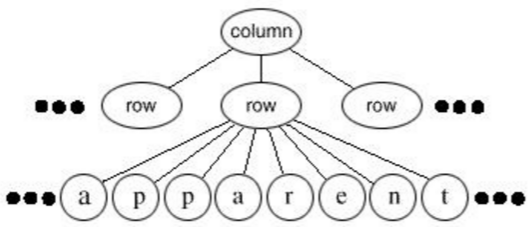
\includegraphics[width=0.38\textwidth]{noFlyweight.png}
            \raisebox{0.1\textheight}{\quad\Huge{$\rightarrow$}\quad}
            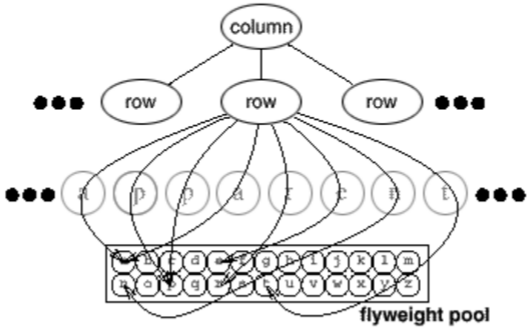
\includegraphics[width=0.38\textwidth]{flyweightExample.png}
        \end{center}
    \end{frame}

    \begin{frame}
        \frametitle{``Приспособленец'', общая схема}
        \begin{center}
            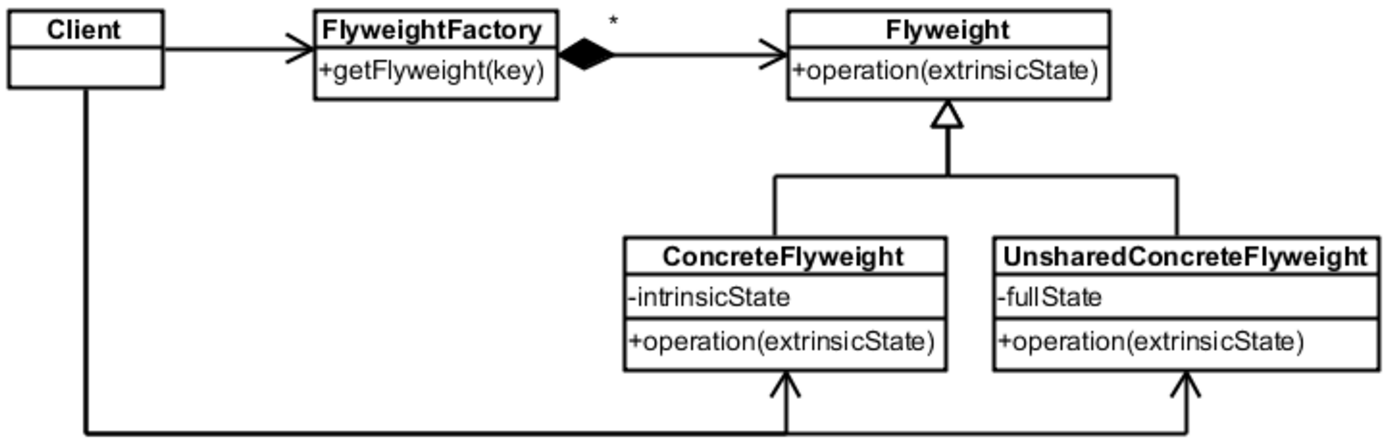
\includegraphics[width=0.7\textwidth]{flyweight.png}
        \end{center}
        \begin{footnotesize}
            \begin{itemize}
                \item \textit{Flyweight} --- определяет интерфейс, через который приспособленцы могут получать внешнее состояние
                \item \textit{ConcreteFlyweight} --- реализует интерфейс Flyweight и может иметь внутреннее состояние, не зависит от контекста
                \item \textit{UnsharedConcreteFlyweight} --- неразделяемый ``приспособленец'', хранящий всё состояние в себе, бывает нужен, чтобы собирать иерархические структуры из Flyweight-ов (``Компоновщик'')
                \item \textit{FlyweightFactory} --- содержит пул приспособленцев, создаёт их и управляет их жизнью
            \end{itemize}
        \end{footnotesize}
    \end{frame}

    \begin{frame}
        \frametitle{``Приспособленец'', диаграмма объектов}
        \begin{center}
            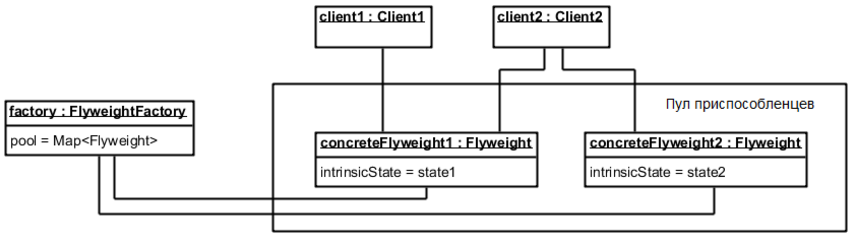
\includegraphics[width=0.7\textwidth]{flyweightObjects.png}
        \end{center}
        \begin{itemize}
            \item Клиенты могут быть разных типов
            \item Клиенты могут разделять приспособленцев
            \begin{itemize}
                \item Один клиент может иметь несколько ссылок на одного приспособленца
            \end{itemize}
            \item Во время выполнения клиенты имеют право не знать про фабрику
        \end{itemize}
    \end{frame}

    \begin{frame}
        \frametitle{Когда применять}
        \begin{itemize}
            \item Когда в приложении используется много мелких объектов
            \item Они допускают разделение состояния на внутреннее и внешнее
            \begin{itemize}
                \item Желательно, чтобы внешнее состояние было вычислимо
            \end{itemize}
            \item Идентичность объектов не важна
            \begin{itemize}
                \item Используется семантика Value Type
            \end{itemize}
            \item Главное, когда от такого разделения можно получить ощутимый выигрыш
        \end{itemize}
    \end{frame}

    \begin{frame}
        \frametitle{Тонкости реализации}
        \begin{itemize}
            \item Внешнее состояние --- по сути, отдельный объект, поэтому если различных внешних состояний столько же, сколько приспособленцев, смысла нет
            \begin{itemize}
                \item Один объект-состояние покрывает сразу несколько приспособленцев
                \begin{itemize}
                    \item Например, объект ``Range'' может хранить параметры форматирования для всех букв внутри фрагмента
                \end{itemize}
            \end{itemize}
            \item Клиенты не должны инстанцировать приспособленцев сами, иначе трудно обеспечить разделение
            \begin{itemize}
                \item Имеет смысл иметь механизм для удаления неиспользуемых приспособленцев
                \begin{itemize}
                    \item Если их может быть много
                \end{itemize}
            \end{itemize}
            \item Приспособленцы немутабельны и Value Objects (с правильно переопределённой операцией сравнения)
            \begin{itemize}
                \item Про hashCode() тоже надо не забыть
            \end{itemize}
        \end{itemize}
    \end{frame}

    \begin{frame}
        \frametitle{Мини-опрос}
        \center{\url{https://forms.gle/S8G2hUehJWL3Y7t36}}
    \end{frame}

    \section{Компоновщик}

    \begin{frame}
        \frametitle{``Компоновщик'' (Composite), детали реализации}
        \begin{columns}
            \begin{column}{0.6\textwidth}
                \begin{itemize}
                    \item Ссылка на родителя
                    \begin{itemize}
                        \item Может быть полезна для простоты обхода
                        \item ``Цепочка обязанностей''
                        \item Но дополнительный инвариант
                        \item Обычно реализуется в Component
                    \end{itemize}
                \end{itemize}
            \end{column}
            \begin{column}{0.4\textwidth}
                \begin{center}
                    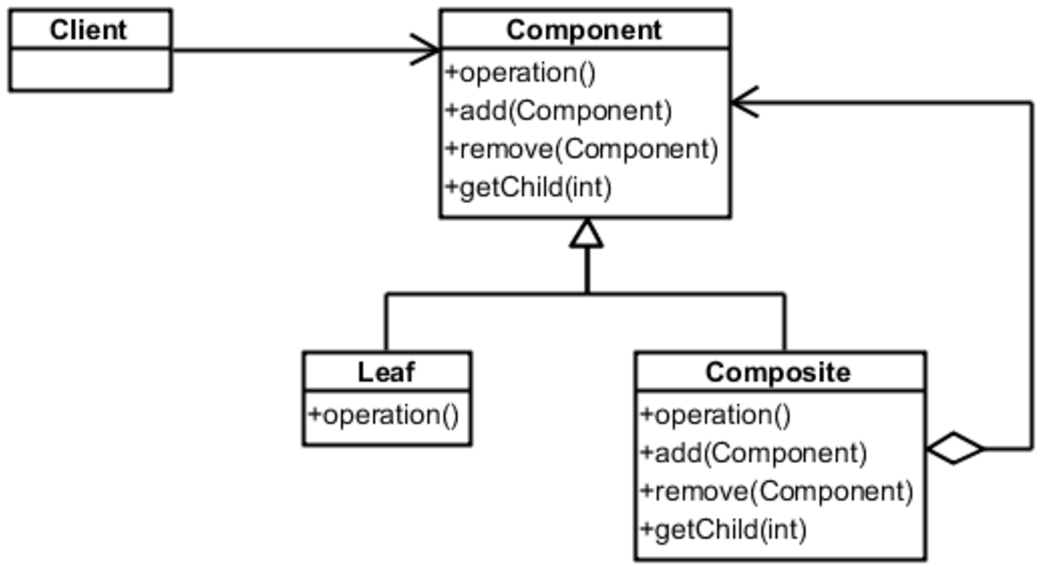
\includegraphics[width=\textwidth]{composite.png}
                \end{center}
            \end{column}
        \end{columns}

        \begin{itemize}
            \item Разделяемые поддеревья и листья
            \begin{itemize}
                \item Позволяют сильно экономить память
                \item Проблемы с навигацией к родителям и разделяемым состоянием
                \item Паттерн ``Приспособленец''
            \end{itemize}
            \item Идеологические проблемы с операциями для работы с потомками
            \begin{itemize}
                \item Не имеют смысла для листа
                \begin{itemize}
                    \item Можно считать Leaf Composite-ом, у которого всегда 0 потомков
                \end{itemize}
                \item Операции add и remove можно объявить и в Composite, тогда придётся делать cast
                \begin{itemize}
                    \item Иначе надо бросать исключения в add и remove
                \end{itemize}
            \end{itemize}
        \end{itemize}
    \end{frame}

    \begin{frame}
        \frametitle{``Компоновщик'', детали реализации (2)}
        \begin{itemize}
            \item Операция getComposite() – более аккуратный аналог cast-а
            \item Где определять список потомков
            \begin{itemize}
                \item В Composite, экономия памяти
                \item В Component, единообразие операций
                \item ``Список'' вполне может быть хеш-таблицей, деревом или чем угодно
            \end{itemize}
            \item Порядок потомков может быть важен, может нет
            \item Кеширование информации для обхода или поиска
            \begin{itemize}
                \item Например, кеширование ограничивающих прямоугольников для фрагментов картинки
                \item Инвалидация кеша
            \end{itemize}
            \item Удаление потомков
            \begin{itemize}
                \item Если нет сборки мусора, то лучше в Composite
                \item Следует опасаться разделяемых листьев/поддеревьев
            \end{itemize}
        \end{itemize}
    \end{frame}

    \section{Декоратор}

    \begin{frame}
        \frametitle{Мини-опрос}
        \center{\url{https://forms.gle/EJjyc3YN7BQwT6b2A}}
    \end{frame}

    \begin{frame}
        \frametitle{``Декоратор'' (Decorator), детали реализации}
        \begin{columns}
            \begin{column}{0.6\textwidth}
                \begin{itemize}
                    \item Интерфейс декоратора должен соответствовать интерфейсу декорируемого объекта
                    \begin{itemize}
                        \item Иначе получится ``Адаптер''
                    \end{itemize}
                    \item Если конкретный декоратор один, абстрактный класс можно не делать
                \end{itemize}
            \end{column}
            \begin{column}{0.4\textwidth}
                \begin{center}
                    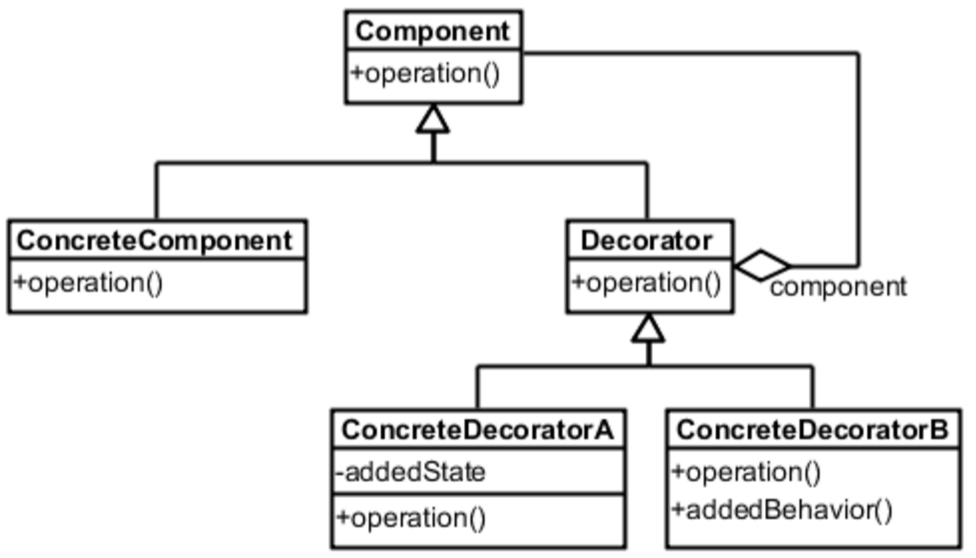
\includegraphics[width=\textwidth]{decorator.png}
                \end{center}
            \end{column}
        \end{columns}
        \begin{itemize}
            \item Component должен быть по возможности небольшим (в идеале, интерфейсом)
            \begin{itemize}
                \item Иначе лучше паттерн ``Стратегия''
                \item Или самодельный аналог, например, список ``расширений'', которые вызываются декорируемым объектом вручную перед операцией или после неё
            \end{itemize}
        \end{itemize}
    \end{frame}

    \section{Стратегия}

    \begin{frame}
        \frametitle{``Стратегия'' (Strategy), детали реализации}
        \begin{center}
            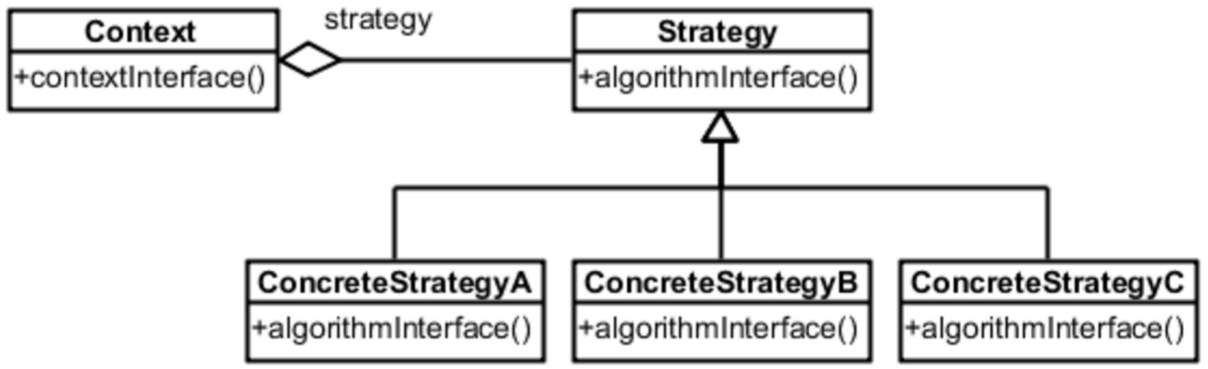
\includegraphics[width=0.6\textwidth]{strategy.png}
        \end{center}
        \begin{itemize}
            \item Передача контекста вычислений в стратегию
            \begin{itemize}
                \item Как параметры метода --- уменьшает связность, но некоторые параметры могут быть стратегии не нужны
                \item Передавать сам контекст в качестве аргумента --- в Context интерфейс для доступа к данным
            \end{itemize}
        \end{itemize}
    \end{frame}

    \begin{frame}
        \frametitle{``Стратегия'' (Strategy), детали реализации (2)}
        \begin{itemize}
            \item Стратегия может быть параметром шаблона
            \begin{itemize}
                \item Если не надо её менять на лету
                \item Не надо абстрактного класса и нет оверхеда на вызов виртуальных методов
            \end{itemize}
            \item Стратегия по умолчанию
            \begin{itemize}
                \item Или просто поведение по умолчанию, если стратегия не установлена
            \end{itemize}
            \item Объект-стратегия может быть приспособленцем
        \end{itemize}
    \end{frame}

    \section{Адаптер}

    \begin{frame}
        \frametitle{``Адаптер'' (Adapter), детали реализации}
        \begin{columns}
            \begin{column}{0.5\textwidth}
                \begin{itemize}
                    \item Адаптер объекта:
                        \vspace{0.3cm}
                        
                        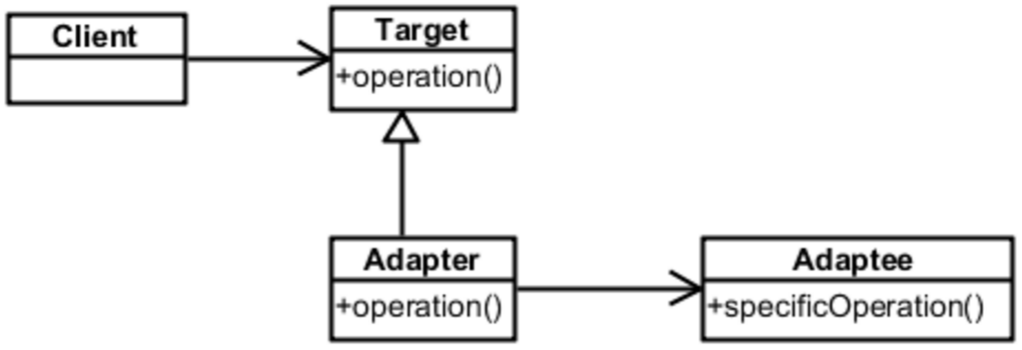
\includegraphics[width=0.8\textwidth]{objectAdapter.png}
                        \vspace{0.3cm}
                    \item Похоже на ``Мост''
                \end{itemize}
            \end{column}
            \begin{column}{0.5\textwidth}
                \begin{itemize}
                    \item Адаптер класса:
                        \vspace{0.3cm}
                        
                        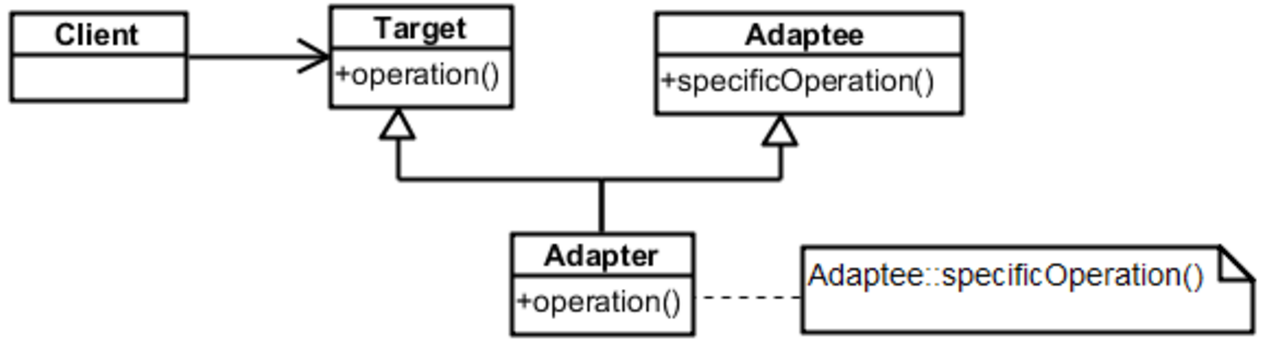
\includegraphics[width=0.9\textwidth]{classAdapter.png}
                        \vspace{0.3cm}
                    \item Нужно множественное наследование
                    \begin{itemize}
                        \item private-наследование в C++
                    \end{itemize}
                \end{itemize}
            \end{column}
        \end{columns}
    \end{frame}

    \section{Фасад}

    \begin{frame}
        \frametitle{``Фасад'' (Facade), детали реализации}
        \begin{columns}
            \begin{column}{0.5\textwidth}
                \begin{itemize}
                    \item Абстрактный Facade
                    \begin{itemize}
                        \item Существенно снижает связность клиента с подсистемой
                    \end{itemize}
                \end{itemize}
            \end{column}
            \begin{column}{0.5\textwidth}
                \begin{center}
                    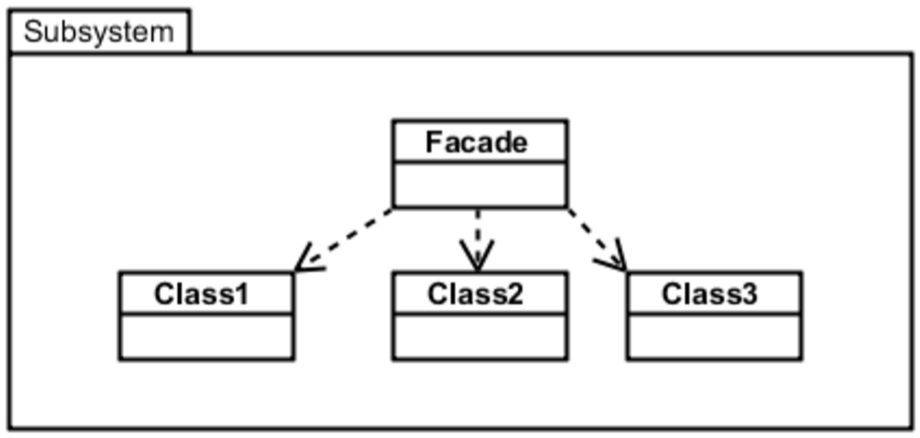
\includegraphics[width=0.8\textwidth]{facade.png}
                \end{center}
            \end{column}
        \end{columns}
        \begin{itemize}
            \item Открытые и закрытые классы подсистемы
            \begin{itemize}
                \item Пространства имён и пакеты помогают, но требуют дополнительных соглашений
                \begin{itemize}
                    \item Пространство имён details
                \end{itemize}
                \item Инкапсуляция целой подсистемы --- это хорошо
            \end{itemize}
        \end{itemize}
    \end{frame}

    \section{Прокси}

    \begin{frame}
        \frametitle{``Заместитель'' (Proxy), детали реализации}
        \begin{center}
            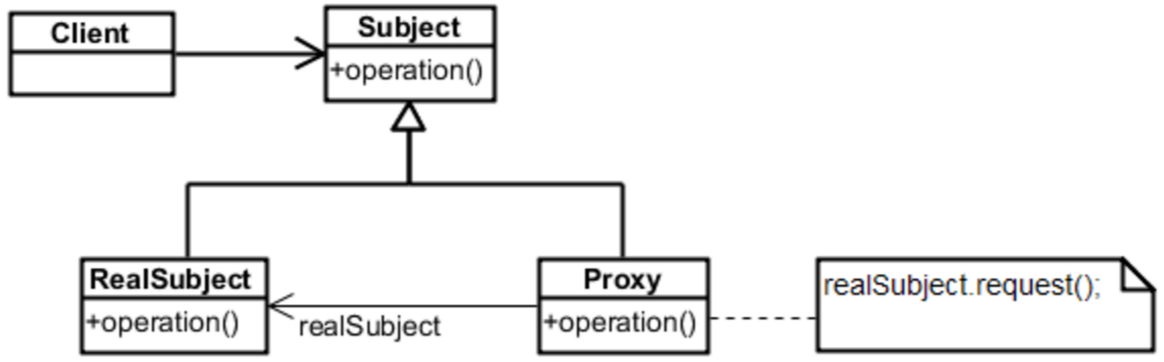
\includegraphics[width=0.7\textwidth]{proxy.png}
        \end{center}
        \begin{itemize}
            \item Перегрузка оператора доступа к членам класса (для C++)
            \begin{itemize}
                \item Умные указатели так устроены
                \item C++ вызывает операторы \mintinline{c++}|->| по цепочке
                \begin{itemize}
                    \item \mintinline{c++}|object->do()| может быть хоть \mintinline{c++}|((object.operator->()).operator->()).do()|
                \end{itemize}
                \item Не подходит, если надо различать операции
            \end{itemize}
        \end{itemize}
    \end{frame}

    \begin{frame}
        \frametitle{``Заместитель'' (Proxy), детали реализации (2)}
        \begin{itemize}
            \item Реализация ``вручную'' всех методов проксируемого объекта
            \begin{itemize}
                \item Сотня методов по одной строчке каждый
                \item C\#/F\#: \mintinline{csharp}|public void do() => realSubject.do();|
                \item Препроцессор/генерация
                \begin{itemize}
                    \item Технологии наподобие WCF
                \end{itemize}
            \end{itemize}
            \item Проксируемого объекта может не быть в памяти
        \end{itemize}
    \end{frame}

    \begin{frame}
        \frametitle{Пример: Apache Thrift}
        \begin{itemize}
            \item Реализация механизма RPC от Facebook
            \item Берёт на себя задачи общения по сети
            \item Сервисы (сигнатуры функций) и используемые типы данных описываются в .thrift-файле
            \item Заглушки (тот самый Proxy) генерятся для 25 языков программирования
        \end{itemize}
    \end{frame}

    \begin{frame}[fragile]
        \frametitle{.thrift}
        \begin{small}
            \begin{minted}{text}
enum PhoneType {
  HOME,
  WORK,
  MOBILE,
  OTHER
}

struct Phone {
  1: i32 id,
  2: string number,
  3: PhoneType type
}

service PhoneSvc {
  Phone findById(1: i32 id),
  list<Phone> findAll()
}
            \end{minted}
        \end{small}
    \end{frame}

    \begin{frame}[fragile]
        \frametitle{Заглушка}
        \begin{small}
            Генерация:

            \mintinline{text}|thrift --gen netcore demo.thrift|

            \vspace{3mm}

            Использование:
        \begin{minted}{csharp}
public static async Task Main(string[] args)
{
    var phone = new PhoneSvc.Client(
        new TBinaryProtocol(
            new TSocketClientTransport(IPAddress.Loopback, 8888)));

    await phone.OpenTransportAsync(CancellationToken.None);
    var allPhones = await phone.findAllAsync(CancellationToken.None);

    foreach (var result in allPhones)
    {
        Console.WriteLine(result);
    }
}
            \end{minted}
        \end{small}
    \end{frame}

    \section{Задание}

    \begin{frame}
        \frametitle{Задание на остаток занятия}
        Спроектировать в рогалике поддержку мобов и боевую систему:
        \begin{itemize}
            \item Несколько разных видов, различающихся характеристиками и поведением
            \begin{itemize}
                \item Агрессивное поведение, атакуют игрока, как только его видят
                \item Пассивное поведение, просто стоят на месте
                \item Трусливое поведение, стараются держаться на расстоянии от игрока
            \end{itemize}
            \item При попытке занять одну клетку существа атакуют друг друга
            \item Использовать паттерн ``Стратегия'' для поддержки различных поведений
            \item Используя паттерн ``Декоратор'', реализовать для игрока возможность конфузить мобов
        \end{itemize}
    \end{frame}

    \begin{frame}
        \frametitle{Организационное}
        \begin{itemize}
            \item У кого проект в онлайн-тулах, расшарьте
            \item Отключаетесь от основного чата и уходите в командный
            \item Ссылку на проект и на командный чат кидаете в \url{https://forms.gle/2nCbEWdavgsk4PhU6}
            \begin{itemize}
                \item Как только ссылки будут готовы, НЕ в конце пары
            \end{itemize}
            \item Посматриваете в конфу в Telegram
            \item За 20 минут до конца пары (в 17:30) сбор в общем чате и представление результатов
            \begin{itemize}
                \item Если все будут готовы раньше, то раньше
            \end{itemize}
        \end{itemize}
    \end{frame}

\end{document}